% !TEX root = main.tex
%----------------------------------------------------------------------
\chapter{Order Statistics}\label{chap:order-statistics}
\setcounter{page}{1}
\startcontents[chapters]
%----------------------------------------------------------------------
\dictum{X}{X}{X}
\chapcontents

%====================================================================
\section{Non-parametric methods}
%====================================================================

A typical problem in statistics is to estimate the distribution of some random variable from a set of observations. 

\vspace*{2ex}
So far we have assumed that the parametric form of the distribution is known:
\bit
\it $X\sim\text{Bernoulli}(\theta)$ where $\theta\in [0,1]$ or $X\sim\text{Poisson}(\theta)$ where $\theta\in(0,\infty)$, etc.
%\it $X\sim\text{Normal}(\mu,\sigma^2)$ where $\mu\in(-\infty,\infty)$ and $\sigma\in(0,\infty)$ are unknown.
\eit

\vspace*{2ex}
We now look at methods for estimating the distribution of a random variable where the parametric form of the distribution is \emph{unknown}.

%Non-parametric tests are used when the conditions of parametric tests are not satisfied.
\bit
\it These are called \emph{non-parametric} or \emph{distribution-free} methods.
%\it Non-parametric methods are used when the conditions for parametric tests are not satisfied.
\eit

\vfill
\begin{minipage}{\linewidth}
\centering
\begin{tabular}{|l||l|}\hline
Parametric methods				& Non-parametric methods \\ \hline\hline
One-sample $t$-test				& The Sign Test \\
Paired samples $t$-test			& The Wilcoxon Signed-Rank Test \\ \hline
Independent samples $t$-test		& The Mann-Whitney Test \\ \hline
One-way ANOVA					& The Kruskal-Wallis Test \\ \hline
%ANOVA for repeated measures 		& The Friedman Test \\
%Pearson Correlation 				& Spearman Rank Order Correlation \\ \hline
\end{tabular}
\end{minipage}

%====================================================================

\section{Order statistics}
%====================================================================
%Let $X_1,X_2,\ldots,X_n$ be an i.i.d.\ random sample from some (unknown) distribution, let $X_{(1)}$ denote the smallest observation, $X_{(2)}$ the second-smallest observation, $\ldots$, $X_{(n-1)}$ the second-largest observation, and $X_{(n)}$ largest observation $X_{(n)}$. 
Let $X_1,X_2,\ldots,X_n$ be an i.i.d.\ random sample from some (unknown) distribution, let $X_{(1)}$ denote the smallest observation, let $X_{(2)}$ denote the second-smallest observation, $\ldots$, and let $X_{(n)}$ denote largest observation: 
\[
X_{(1)} \leq X_{(2)} \leq \ldots \leq X_{(n)}
\]
%Then $X_{(1)} \leq X_{(2)} \leq \ldots \leq X_{(n)}$.

% defn: order statistics
\begin{definition}
$X_{(1)}, X_{(2)}, \ldots, X_{(n)}$ are called the \emph{order statistics} of the random sample $X_1,X_2,\ldots,X_n$.
\end{definition}

Some functions of the order statistics are important statistics in their own right:
\bit
\it The \emph{sample minimum} is $X_{(1)}$ and the \emph{sample maximum} is $X_{(n)}$.
\it The \emph{sample range} is $R = X_{(n)} - X_{(1)}$.
\it The \emph{sample median} is $M = \begin{cases} X_{(n/2+1/2)} & \quad\text{if $n$ is odd,} \\[2ex] \frac{1}{2}X_{(n/2)}+\frac{1}{2}X_{(n/2+1)} & \quad\text{if $n$ is even.} \end{cases}$
\eit
\vspace*{-2ex}
% remark: expensive
\begin{remark}
Computing order statistics involves sorting the data, which may be computationally expensive.
\end{remark}

%--------------------------------------------------

\section{Quantiles}
%--------------------------------------------------
Let $X$ be a continuous random variable and let $F(x)$ denote its CDF.

% defn: quantile
\begin{definition}
For $0<p<1$, the \emph{$p^{\text{th}}$ quantile} of $X$ is defined by $\xi_p = F^{-1}(p)$.
\end{definition}

%In particular,
\begin{hidebox}
\bit
\it $\xi_{0.5}$ is the \emph{median}.
\it $\xi_{0.25}$ is the \emph{lower quartile}.
\it $\xi_{0.75}$ is the \emph{upper quartile}.
\it $\xi_{0.75}-\xi_{0.25}$ is the \emph{inter-quartile range}.
\eit
\end{hidebox}

%% sketch
%
%\picbox[Quantiles]{5cm}

% remark: location and scale
\begin{remark}
\bit
\it The median quantifies the \emph{location} of a distribution.
\it The inter-quartile range quantifies the \emph{scale} of a distribution.
\eit
\end{remark}

\subsection{Sample quantiles}
% defn: sample quantile
\begin{definition}
Let $X$ be a continuous random variable, let $X_{(1)},X_{(2)},\ldots,X_{(n)}$ be the order statistics of a random sample from the distribution of $X$, and let $p\in(0,1)$. The $p^{\text{th}}$ \emph{sample quantile} of $X$ is defined by the weighted average
\[
\hat{\xi}_p = \big(1-\{k\}\big)X_{([k])} + \{k\}X_{([k]+1)}
\]
where $k=(n+1)p$.
\end{definition}

\begin{remark}
\bit
\it $[k]$ and $\{k\}$ are the integer and fractional parts of $k$, respectively.
\it If $k=(n+1)p$ is an integer, the sample quantile $\hat{\xi}_p$ is simply $X_{(k)}$.
\eit
\end{remark}

 % <<

% example: sample quantile
\begin{example}
Let $1,7,4,3$ be a random sample from some unknown distribution. 

\ben
\it What is the $0.6^{\text{th}}$ sample quantile of the distribution?
\it What is the $0.65^{\text{th}}$ sample quantile of the distribution?
\een
\end{example}

\begin{solution}
The observed order statistics are $x_{(1)}=1$, $x_{(2)}=3$, $x_{(3)}=4$ and $x_{(4)}=7$.

\ben
\it 
For $p=0.6$ we have $k=(n+1)p = 5\times 0.6 = 3$. 
\par
In this case, $[k]=3$ and $\{k\}=0$, so 
\[
\hat{\xi}_{0.6} = x_{(3)} = 4.
\]

\it
For $p=0.65$ we have $k=(n+1)p = 5\times 0.65 = 3.25$. 
\par
In this case, $[k]=3$ and $\{k\}=0.25$, so 
\[
\hat{\xi}_{0.65} = (1-0.25)\times x_{(3)} + 0.25\times x_{(4)} = 4.75.
\]
\een
\end{solution}

%--------------------------------------------------

\section{Q-Q plots}
%--------------------------------------------------
%We consider the \emph{location-scale} family of distributions. 
%A \emph{location-scale} model is a family of distributions parametrized by a location parameter and a non-negative scale parameter;
\bit
\it Let $Z$ be a random variable, and let $F(z)$ denote its CDF.
\it Let $Y = a + bZ$, where $a$ and $b>0$ are unknown.
\eit
The CDF of $Y$ is 
\[
\prob(Y\leq y) 
	= \prob\left(Z\leq\frac{y-a}{b}\right) = F\left(\frac{y-a}{b}\right).
\]
\bit
\it Suppose we wish to test whether the CDF of $X$ is of the form $\displaystyle F\left(\frac{x-a}{b}\right)$.
\eit

%Let $X$ be a  RV with distribution function $\displaystyle F\left(\frac{x-a}{b}\right)$ where $F$ is known, but $a$ and $b>0$ are unknown.
%
%Then $Z = \displaystyle\frac{X-a}{b}$ has distribution function $F(z)$.

Let $\xi_p^{(Z)}$ and $\xi_p^{(X)}$ denote the $p^{\text{th}}$ quantiles of $Z$ and $X$ respectively (where $0<p<1$).
%\bit
%\it let $\xi_p^{(Z)}$ denote the $p^{\text{th}}$ quantile of $Z$, and let $\xi_p^{(X)}$ denote the $p^{\text{th}}$ quantile of $X$.
%\eit

\vspace*{2ex}
\bit
\it $\xi_p^{(Z)} = F^{-1}(p)$ is known
\it $\xi_p^{(X)} = a + bF^{-1}(p)$ is unknown.
\eit

\vspace*{2ex}
If the CDF of $X$ is indeed of the form $\displaystyle F\left(\frac{x-a}{b}\right)$ we have the linear relationship 
\[
\xi_p^{(X)} = a + b\,\xi_p^{(Z)}.
\]

%\bit
%\it The quantiles of $X$ can be estimated by the order statistics of a random sample from its distribution.
%\it This yields a test of whether $X$ is a member of the so-called \emph{location-scale} family of distributions defined by $Z$.
%\eit

%Since $p = F(\xi_p^{(Z)})$ and $p = \displaystyle F\left(\frac{\xi_p^{(X)} - a}{b}\right)$, we have the linear relationship 
%\[
%\xi_p^{(X)} = a + b\,\xi_p^{(Z)}
%\]
%provided the distribution function of $X$ is indeed of the form $\displaystyle F\left(\frac{x-a}{b}\right)$.
%\bit
%\it The quantiles $\xi_p^{(X)}$ of $X$ are unknown, but we can estimate them.
%\eit

 % <<

Although the quantiles $\xi_p^{(X)}$ of $X$ are unknown, they can be estimated using order statistics.

\vspace*{1ex}
\bit
\it Let $X_1,X_2,\ldots,X_n$ be a random sample from the distribution of $X$.
\it Let $X_{(1)},X_{(2)},\ldots,X_{(n)}$ be the order statistics of $X_1,X_2,\ldots,X_n$.
\it $X_{(k)}$ is a point estimator of $\xi_{p_k}^{(X)}$, where $p_k=k/(n+1)$.
\eit

\vspace*{3ex}
The plot of $X_{(k)}$ against $\xi_{p_k}^{(Z)}$ is called a \emph{Quantile-Quantile plot} (or Q-Q plot).

\vspace*{2ex}
\bit
\it If the CDF of $X$ is indeed of the form $\displaystyle F\left(\frac{x-a}{b}\right)$, the plot should be approximately linear.
\it The unknown parameters $a$ and $b$ can be estimated by the intercept and gradient of the plot, respectively.
\eit


 % <<

\begin{example}
To test whether a random sample $X_1,X_2,\ldots,X_n$ is from a Normal distribution, we plot the order statistics $X_{(k)}$ against $\Phi^{-1}\big[k/(n+1)\big]$ for $k=1,2,\ldots,n$. 
\bit
\it If the points lie on a straight line, we may conclude that the $X_i$ are normally distributed. %indeed normally distributed. 
\it Such plots are often called \emph{Normal Q-Q plots}.
\eit
\begin{minipage}{\linewidth}
\begin{minipage}{0.45\linewidth}
\resizebox{\linewidth}{!}{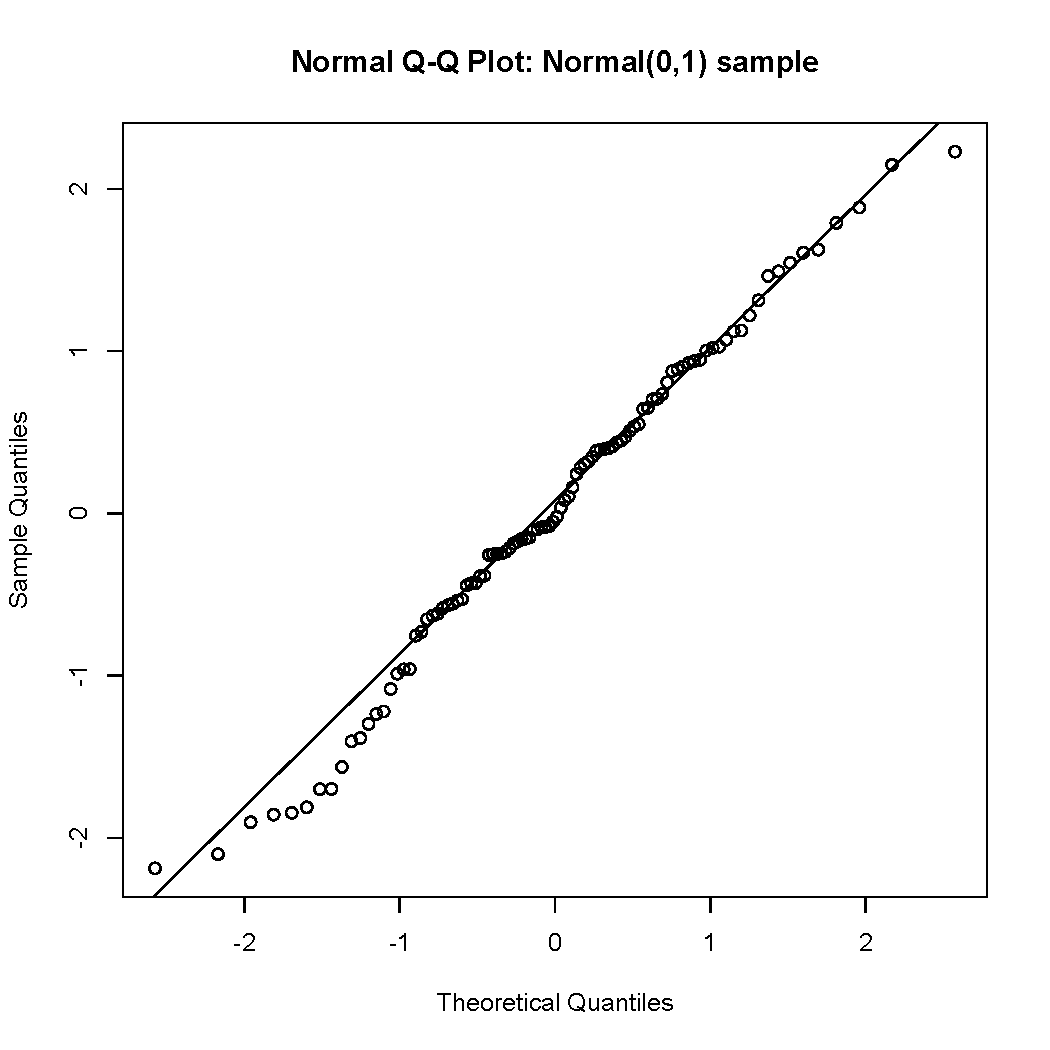
\includegraphics{nqqplot-normal}}
\end{minipage}
\hfill
\begin{minipage}{0.45\linewidth}
\resizebox{\linewidth}{!}{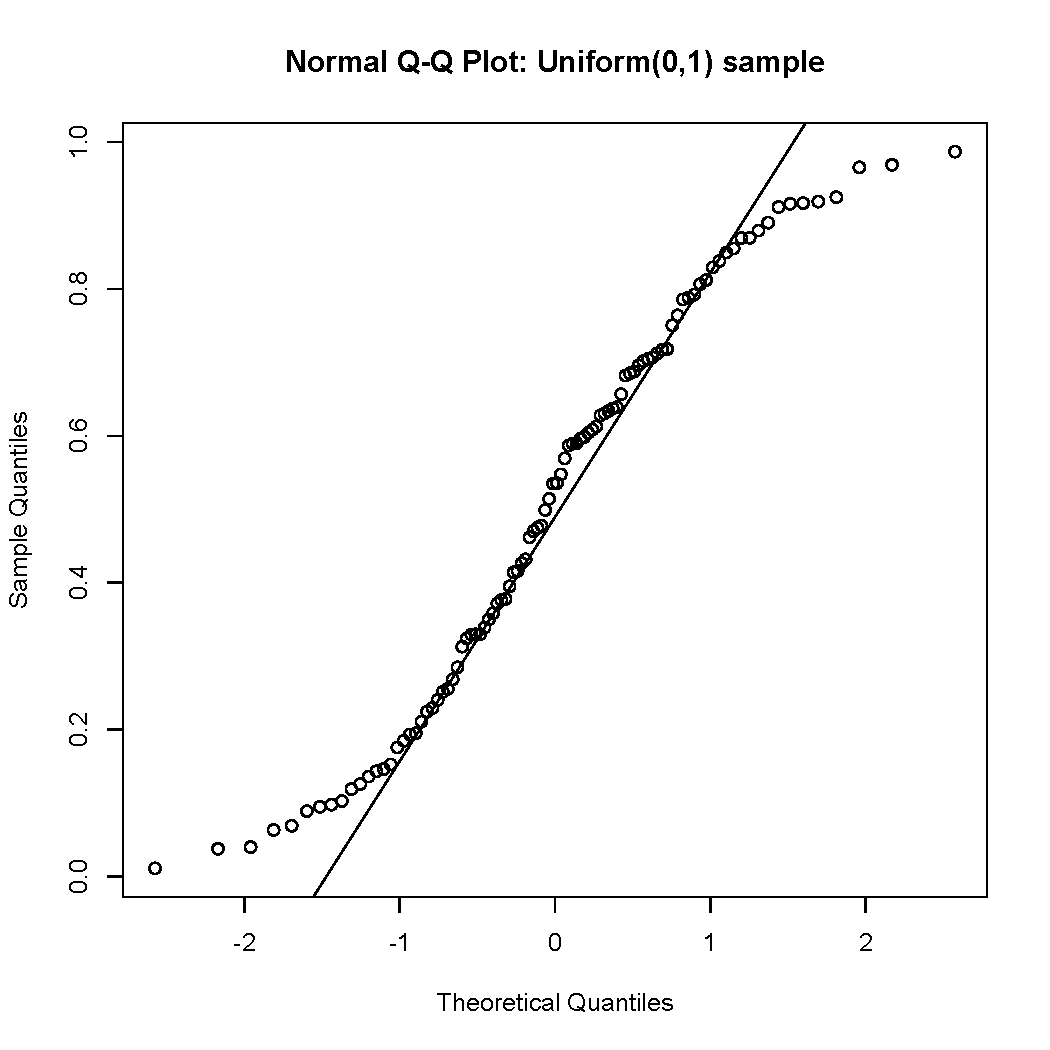
\includegraphics{nqqplot-uniform}}
\end{minipage}
\end{minipage}
\end{example} 

%%--------------------------------------------------
%
%\section{Confidence intervals for quantiles}
%%--------------------------------------------------
%Let $X$ be a continuous random variable with distribution function $F(x)$, and let $X_{(1)},X_{(2)},\ldots,X_{(n)}$ denote the order statistics of an i.i.d.\ random sample of size $n$ from the distribution of $X$. 
%\bit
%\it If $k=[(n+1)p]$, the $k^{\text{th}}$ order statistic $X_{(k)}$ is a point estimate of $\xi_p$.
%\eit
%To derive an \emph{interval estimate} of $\xi_p$, consider the event $\{X_{(i)} < \xi_p < X_{(j)}\}$. 
%
%If this event occurs, then 
%\bit
%\it at least $i$ sample points are smaller than $\xi_p$, 
%\it at most $j-1$ sample points are smaller than $\xi_p$.
%\eit
%
%Thus the event $\{X_{(i)} < \xi_p < X_{(j)}\}$ is equivalent to observing between $i$ and $j-1$ successes in $n$ independent Bernoulli trials, where the probability of success is $p = \prob(X\leq \xi_p) = F(\xi_p)$, so 
%\[
%\prob(X_{(i)} < \xi_p < X_{(j)}) = \sum_{w=i}^{j-1}\binom{n}{w} F(\xi_p)^w\big[1-F(\xi_p)\big]^{n-w}.
%\]
%
%\bit
%\it Suppose we find that $\prob(X_{(i)} < \xi_p < X_{(j)}) = 1-\alpha$.
%\it Then the interval $\big(X_{(i)},X_{(j)}\big)$ is a $100(1-\alpha)\%$ confidence interval for $\xi_p$.
%\eit
%
%% example
%\begin{example}[CI for median]
%Let $X$ be a continuous random variable with distribution function $F(x)$, and let $X_{(1)},X_{(2)},\ldots,X_{(n)}$ denote the order statistics of a random sample from the distribution of $X$. 
%\bit
%\it
%The sample median $M$ is an estimate of the true median $\xi_{0.5}$. 
%\it
%For $0<\alpha<1$, let $c_{\alpha/2}$ be such that $\prob\big[X_{(c_{\alpha/2}+1)} < \xi_{0.5} < X_{(n-c_{\alpha/2})}\big] = 1-\alpha$.
%\it
%The value $c_{\alpha/2}$ is found using tables of the $\text{Binomial}(n,p)$ distribution: for the median, we need $p=0.5$.
%\eit
%\end{example}
%
% % <<
%
%% example
%\begin{example}
%The following data are an ordered realisation of a random sample from an unknown distribution.
%\[\begin{array}{ccccccccccccccc}
%56 & 70 & 89 & 94 & 96 & 101 & 102 & 102 & 102 & 105 & 106 & 108 & 110 & 113 & 116 \\
%\end{array}\]
%Find an $88\%$ confidence interval for the median $\xi_{0.5}$ of the distribution.
%\end{example}
%
%\begin{solution}
%\bit
%\it $88\% = (1-\alpha)100\% \quad\Rightarrow\quad \alpha/2=0.06$.
%\it From tables, $\prob\big[\text{Binomial}(15,0.5)\leq 4\big] = 0.059$, so we take $c_{\alpha/2}=4$.
%\it Hence an $88\%$ confidence interval for the median is $(x_{(5)},x_{(11)}) = (96,106)$.
%\eit
%\end{solution}
%====================================================================
\section{The Median}
%====================================================================
The methods we shall consider are based on the \emph{median} of the distribution under investigation.

\vspace*{1ex}
Let $X$ be a random variable.% and let $F$ denote its CDF.

\ben
\it A median $\eta$ of $X$ satisfies the inequalities
\[
\prob(X\leq\eta)\,\geq\frac{1}{2} \quad\text{and}\quad \prob(X\geq\eta)\,\geq\frac{1}{2}.
\]
\it If $X$ is a continuous random variable, its median is uniquely defined and satisfies
\[
\prob(X\leq\eta) = \prob(X\geq\eta) = \frac{1}{2}.
\]
\een

\begin{example}
Consider the random sample $\{1, 2, 2, 2, 3, 14\}$.
\bit
\it Sample median: $\hat{\eta} = 2$.
\it Sample mean:   $\hat{\mu}  = 4$.
\eit
In this case, $\hat{\eta}$ provides a better indicator of centrality than $\hat{\mu}$.
\end{example}

\begin{remark}
\bit
\it The mean $\mu$ minimizes the sum of squared deviations,
\[
\mu = \arg\min_c\sum_{i=1}^n (X_i-c)^2
\]
\it The median $\eta$ minimizes the sum of absolute deviations,
\[
\eta = \arg\min_c\sum_{i=1}^n |X_i-c|
\]
\it If the probability distribution is \emph{symmetric}, the median coincides with the mean.
\eit
\end{remark}

%======================================================================
\endinput
%======================================================================

%====================================================================
%====================================================================
\lecture[31]{The Sign Test}
%====================================================================
%====================================================================

For a random sample $X_1, X_2, . . . , X_n$ of observations from a distribution with (unknown) median $\eta$, the \emph{sign test} evaluates the null hypothesis $H_0:\eta=\eta_0$ against a suitable alternative. To apply the sign test, we need that
%
%
%\begin{align*}
%H_0:\ & \eta = \eta_0 \\
%H_1:\ & \eta \neq \eta_0 \\
%\end{align*}
%
\ben
\it the distribution is continuous,
\it the observations can be ranked, and
\it the observations are independent.
\een
%If we want to evaluate a hypothesized mean ($\mu_0$), we must also assume that 
%\bit
%\it The distribution is symmetric.
%\eit

%\subsection*{The Basic Idea}
The test statistic $S^{+}_n$ is the number of observations that are greater than $\eta_0$: 
\[
S^{+}_n = \sum_{i=1}^n I(X_i>\eta_0) 
\]
We also define the complementary statistic $S^{-}_n = \displaystyle\sum_{i=1}^n I(X_i<\eta_0)$, and note that $S^{+}_n + S^{-}_n = n$.

Under $H_0:\eta=\eta_0$, the distribution of the test statistic is $S^{+}_n\sim\text{Binomial}(n,1/2)$.

%Under the null hypothesis, $S^{+}$ has binomial distribution with parameters $n$ and $p=0.5$.
%\bit
%\it  so $S^{+}\sim\text{Binomial}(n,0.5)$ under $H_0$.
%\eit

\bit
%\it Under $H_0:\eta=\eta_0$, we expect half of the observations to be bigger than $\eta_0$. 
%\it $S^{+}_n$ small suggests that $\eta < \eta_0$;\quad $S^{+}_n$ large suggests that $\eta > \eta_0$.
\it $S^{+}_n$ small suggests that $\eta < \eta_0$.
\it $S^{+}_n$ large suggests that $\eta > \eta_0$.
\eit

%Under the null hypothesis, $S^{+}$ has binomial distribution with parameters $n$ and $p=0.5$.
%\bit
%\it $\prob_{H_0}(X_i>\eta_0)=0.5$ so $S^{+}\sim\text{Binomial}(n,0.5)$ under $H_0$.
%\eit

To perform the sign test we assume that $S^{+}_n\sim\text{Binomial}(n,\theta)$, and test $H_0:\theta = 0.5$ against a suitable alternative, for example $H_1:\theta\neq 0.5$. 


% example: sign test (one sample)
\begin{example}[Sign test]
The following are measurements of the breaking strength of a certain kind of two-inch cotton ribbon.
\[\begin{array}{cccccccccc}
163 & 165 & 160 & 189 & 161 & 171 & 158 & 151 & 169 & 162 \\
163 & 139 & 172 & 165 & 148 & 166 & 172 & 163 & 187 & 173 \\
\end{array}\]
Use the sign test to evaluate $H_0:\eta=160$ against $H_1:\eta>160$ at significance level $\alpha=0.05$.
\end{example}

\begin{solution}
Assume that the population is continuous. 
\small
\[\begin{array}{cccccccccc} \hline
163 & 165 & 160 & 189 & 161 & 171 & 158 & 151 & 169 & 162 \\
+ & + & 0 & + & + & + & - & - & + & + \\ \hline
163 & 139 & 172 & 165 & 148 & 166 & 172 & 163 & 187 & 173 \\
+ & - & + & + & - & + & + & + & + & + \\ \hline
\end{array}\]
 Nmalsize
We have $n=19$ signs (one discarded) and the test statistic $S^{+}_n=15$. 
\par
Under the null hypothesis, $S^{+}_n\sim\text{Binomial}(19,1/2)$. 
\par
From tables, we find that $\prob_{H_0}(S^{+}_n\geq 15) = 0.0095$. 
\par
Thus we reject $H_0$ at significance level $\alpha=0.05$.
\end{solution}

% example: sign test (paired samples)
\begin{example}[Sign test for paired samples]
To evaluate a new traffic-control system, the number of accidents that occurred at 12 dangerous junctions were recorded during the four weeks prior to the installation of the new system, and for the four weeks after its installation. The following data were obtained.
\[\begin{array}{|l|rrrrrrrrrrrr|} \hline
\text{Junction}	& \phantom{1}1 & \phantom{1}2 & \phantom{1}3 & \phantom{1}4 & \phantom{1}5 & \phantom{1}6 & \phantom{1}7 & \phantom{1}8 & \phantom{1}9 & 10 & 11 & 12 \\ \hline
\text{Before}	& 3 & 5 & 2 & 3 & 3 & 3 & 0 & 4 & 1 &  6 &  4 &  1 \\
\text{After}		& 1 & 2 & 0 & 2 & 2 & 0 & 2 & 3 & 3 &  4 &  1 &  0 \\ \hline
\end{array}\]
Use the sign test to decide whether or not the new system is more effective than the old system.
\end{example}

\begin{solution}
Let $\eta_1$ and $\eta_2$ denote the (true) median number of accidents before and after the new system was installed, respectively. We test $H_0:\eta_1=\eta_2$ against $H_1:\eta_1 > \eta_2$.
\[\begin{array}{|l|rrrrrrrrrrrr|} \hline
\text{Junction}	& \phantom{1}1 & \phantom{1}2 & \phantom{1}3 & \phantom{1}4 & \phantom{1}5 & \phantom{1}6 & \phantom{1}7 & \phantom{1}8 & \phantom{1}9 & 10 & 11 & 12 \\ \hline
\text{Before}		& 3 & 5 & 2 & 3 & 3 & 3 & 0 & 4 & 1 &  6 &  4 &  1 \\
\text{After}			& 1 & 2 & 0 & 2 & 2 & 0 & 2 & 3 & 3 &  4 &  1 &  0 \\ \hline
\text{Difference}	& + & + & + & + & + & + & - & + & - &  + &  + &  + \\ \hline
\end{array}\]

%\par\centering
%\begin{tabular}{|l|cccccccccccc|} \hline
%Junction		& 1 & 2 & 3 & 4 & 5 & 6 & 7 & 8 & 9 & 10 & 11 & 12 \\ \hline
%Before		& 3 & 5 & 2 & 3 & 3 & 3 & 0 & 4 & 1 &  6 &  4 &  1 \\
%After		& 1 & 2 & 0 & 2 & 2 & 0 & 2 & 3 & 3 &  4 &  1 &  0 \\ \hline
%Difference	& + & + & + & + & + & + & - & + & - &  + &  + &  + \\ \hline
%\end{tabular}
%\flushleft\par
We have $n=12$, and the value of the test statistic is $S^{+}_n = 10$, where $S^{+}_n\sim\text{Binomial}(12,\theta)$.
\par
Under $H_0:\theta=0.5$, from tables we obtain $\prob_{H_0}(S^{+}_n\geq 10) = 0.0192 < 0.05$.
\par
Thus we conclude that the new system has reduced the number of accidents at dangerous junctions.
\end{solution}

%============================= 
\subsection{Normal approximation}
%============================= 
Recall that if $X\sim\text{Binomial}(n,p)$ then $X\sim N\big(np,np(1-p)\big)$ approx. for $n$ sufficiently large.

For large samples ($n\geq 10$), the test statistic $S^{+}_n$ thus has approximate distribution $S^{+}_n\sim N(n/2,n/4)$ under the null hypothesis $H_0:\theta=1/2$ .

Because we are approximating a discrete distribution by a continuous distribution, we replace $S^{+}_n$ by $S^{+}_n-1/2$, and compute the test statistic
\[
Z = \frac{[S^{+}_n-1/2] - n/2}{\sqrt{n}/2} \sim N(0,1)\quad\text{approx. for $n$ sufficiently large.}
\]
\begin{remark}
Using $S^{+}_n-1/2$ instead of $S^{+}_n$ is known as the \emph{continuity correction}.
\end{remark}


% example: sign test (large sample)
\begin{example}[Sign test for large samples]
The following data are the amounts of sulphur oxide (in tons) emitted by a large industrial plant over a period of 40 days.
\[\begin{array}{cccccccccc}
17 & 15 & 20 & 29 & 19 & 18 & 22 & 25 & 27 &  9 \\
24 & 20 & 17 &  6 & 24 & 14 & 15 & 23 & 24 & 26 \\
19 & 23 & 28 & 19 & 16 & 22 & 24 & 17 & 20 & 13 \\
19 & 10 & 23 & 18 & 31 & 13 & 20 & 17 & 24 & 14
\end{array}\]
Use the sign test to evaluate $H_0:\eta=21.5$ against $H_1:\eta<21.5$ at significance level $\alpha=0.01$.
\end{example}

\begin{solution}
Assume that sulphur oxide emissions per day has continuous distribution.

The test statistic is $S^{+}_n = \sum_{i=1}^n I(X_i > \eta_0) \sim \text{Bin}(n,\theta)$.

Since the sample is relatively large, $S^{+}_n\sim N\big(n\theta,n\theta(1-\theta)\big)$ approx.

Using the continuity correction (for a a lower-tailed test), the test statistic is $Z = \displaystyle\frac{(S^{+}_n+1/2)-n\theta}{\sqrt{n\theta(1-\theta)}}$.

Here, we have $n=40$ and $S^{+}_n=16$ (the number values exceeding $\mu_0 = 21.5$). 

Under $H_0:\theta=1/2$, the value of the test statistic is
\[
z = \frac{16.5 - 20}{\sqrt{10}} = -1.1068.
\]
From tables, the critical value (for a lower-tailed test) is $z_c = \Phi^{-1}(0.01) = -2.33$ (approx). Thus we do not reject $H_0$, and conclude that the median amount of sulphur dioxide emitted by the plant is not less than $21.5$ tons per day.
\end{solution}

%====================================================================
%====================================================================
\lecture[32]{The Wilcoxon signed rank test}
%====================================================================
%====================================================================

%====================================================================
\section{Ranks}
%====================================================================

\begin{definition}
For a random sample $X_1,\ldots,X_n$, the \emph{rank} of observation $X_i$ is its position in the sequence of observations, sorted in ascending order:
\[
R(X_i) = \sum_{j=1}^n I(X_j \leq X_i)
\]
\end{definition}
Note that $\displaystyle\sum_{i=1}^n R(X_i) = \frac{1}{2}n(n+1)$.

In non-parametric tests based on ranks,
\bit
\it similar numbers of high and low ranks across groups $\Rightarrow$ groups are similar.
\it different numbers of high and low ranks across groups $\Rightarrow$ groups are different.
\eit

%============================= 
\subsection{Ties}
%============================= 

\bit
\it The distribution is assumed to be continuous, so ties should occur with probability zero.
\it Ties often occur in practical applications however, due to the limited precision of measurements.
\it The simplest way to deal with ties is to assign an average rank to each of the tied observations.
\eit

For example, if there are $m-1$ observations strictly smaller than $X_i=X_j$, we set
\[
R(X_i) = R(X_j) = \frac{m+(m+1)}{2} = m+\frac{1}{2}
\]

%====================================================================
\section{The WSR test}
%====================================================================
The \emph{Wilcoxon signed rank test} is a refinement of the sign test.
%\bit
%\it The WSR test is a non-parametric version of the one-sample $t$-test and paired-samples $t$-test.
\bit
\it The sign test counts the number observations above (or below) the hypothesized median.
\it The WSR test sums the ranks of observations above (or below) the hypothesized median.
\eit
%\eit
%\begin{align*}
%H_0:\ & \eta = \eta_0 \\
%H_1:\ & \eta \neq \eta_0 \qquad\text{(or $H_1:\eta<\eta_0$, or $H_1:\eta>\eta_0$)}
%\end{align*}
To apply the WSR test, we require the following conditions:
\ben
\it the distribution is continuous and symmetric (around its mean),
\it the observations can be ranked, and
\it the observations are independent.
\een

\begin{remark}
If the density of a distribution is symmetric, its mean and median coincide.
\end{remark}

\bit
\it Without loss of generality, we consider the null hypothesis $H_0:\eta=0$ against a suitable alternative.
\it For the general case $H_0:\eta=\eta_0$, we simply consider the sample $X_1-\eta_0,\ldots,X_n-\eta_0$.
\eit

% definition: wsr statistic
\begin{definition}
Let $X_1,X_2,\ldots,X_n$ be an i.i.d.\ random sample from a continuous and symmetric distribution, with (unknown) median $\eta$. For the null hypothesis $H_0:\eta=0$, the \emph{Wilcoxon signed rank} (WSR) statistic is defined to be
\[
W^{+}_n = \sum_{i=1}^n R_i Z_i \quad\text{where}\quad R_i = \sum_{j=1}^n I(|X_j|\leq |X_i|) \quad\text{and}\quad Z_i=I(X_i>0).
\]
\end{definition}

% remarks
\bit
\it $R_i$ is the rank of $|X_i|$ in the sample of absolute values $|X_1|,|X_2|,\ldots,|X_n|$.
\it $Z_i=1$ if $X_i>0$, otherwise $Z_i=0$.
\eit

%We also define the complementary statistic $W^{-}_n = \displaystyle\sum_{i=1}^n R(|X_i|) I(X_i<0)$. 
We also define the complementary statistic $W^{-}_n = \displaystyle\sum_{i=1}^n R_i(1-Z_i)$, and note that
\[
W^{+}_n + W^{-}_n = \sum_{i=1}^n R_i = \sum_{i=1}^n i = \frac{1}{2}n(n+1).
\]

% test procedure
In practice, the WSR test procedure is as follows:
\ben
\it Compute the differences $D_i = X_i - \eta_0$ (single sample) or $D_i=X_i-Y_i$ (matched pairs).
\it Compute absolute differences $|D_i|$ and record the sign of $D_i$.
\it Compute the ranks $R_i$ of the absolute differences $|D_i|$.
\it Compute the the sum of the ranks of those $|D_i|$ having positive sign (this is the test statistic $W^{+}$).
\een

% example
\begin{example}
A study of the effects of smoking by mothers on the birthweight of their children involved 12 pairs of mothers. The pairs of mothers were selected so that they were as similar as possible, except that one mother of each pair was a smoker and the other was not. The birthweights (in kilograms) of the babies were as follows.
\[\begin{array}{l|cccccccccccc} \hline
\text{Pair}			& 1      &  2     & 3      & 4      & 5      & 6      & 7      & 8      & 9      & 10     & 11     & 12 		\\ \hline
\text{Non-smoker}	& 3.22   & 4.48   & 3.90   & 3.47   & 3.07   & 3.23   & 4.25   & 3.31   & 3.33   & 3.78   & 3.18   & 4.60  	\\ 
\text{Smoker}		& 3.00   & 4.27   & 3.95   & 3.32   & 2.51   & 2.77   & 4.02   & 3.41   & 3.39   & 3.88   & 3.18   & 4.37 	\\ \hline
\end{array}\]
Do these data conform with the hypothesis that mothers who smoke tend to have babies with smaller birthweights than those who do not? 
\end{example}

\begin{solution}
The data are in matched pairs so we compute the differences $D_i=X_i-Y_i$, and evaluate
\[
H_0:\eta = 0 \quad\text{against}\quad H_1:\eta > 0,
\]
where $\eta$ is the (true) median difference between birthweights for the non-smoking group and birthweights for the smoking group.
\[\begin{array}{|c|cccccccccccc|} \hline
i			& 1      &  2     & 3      & 4      & 5      & 6      & 7      & 8      & 9      & 10     & 11     & 12   	\\ \hline
X_i			& 3.22   & 4.48   & 3.90   & 3.47   & 3.07   & 3.23   & 4.25   & 3.31   & 3.33   & 3.78   & 3.18   & 4.60 	\\ 
Y_i			& 3.00   & 4.27   & 3.95   & 3.32   & 2.51   & 2.77   & 4.02   & 3.41   & 3.39   & 3.88   & 3.18   & 4.37	\\ \hline
D_i			& 0.22   & 0.21   & -0.05  & 0.15   & 0.56   & 0.46   & 0.23   & -0.10  & -0.06  & -0.10  & 0.00  	& 0.23	\\
\text{sgn}(D_i)	& +      & +      & -      & +      & +      & +      & +      & -      & -      & -      &      	& +  	\\ \hline
|D_i|		& 0.22   & 0.21   &  0.05  & 0.15   & 0.56   & 0.46   & 0.23   &  0.10  &  0.06  &  0.10  & 0.00  	& 0.23	\\
R(|D_i|)		& 8      & 7      & 2      & 6      & 12     & 11     & 9.5    &  4.5   &  3     &  4.5   & 0     	& 9.5  	\\ \hline
\end{array}\]
\bit
\it There is a zero difference: this is discarded, leaving $n=11$ non-zero differences.
\it Ties are replaced by the average of the corresponding ranks.
\eit
From the data, $W^{+}_n = 56$ and $W^{-}_n = 10$. \qquad Check:\quad $W^{+}_n + W^{-}_n = 66 = \frac{1}{2}n(n+1)$. 
\par
A large positive value of $W^{+}_n$ supports the alternative hypothesis, $H_1:\eta > 0$. 
\par
From tables, the critical value of $W^{+}_n$ for $n=11$ at $\alpha=0.05$ is $w_c = 52$. 
\par
Since $W^{+}_n > w_c$, we reject the null hypothesis and conclude that the data support the hypothesis that mothers who smoke tend to have babies with smaller birthweights than those who do not. 
\end{solution}

%%==========================================================================
%\begin{example}
%The data below are a random sample from a symmetric continuous random variable  with mean equal to $\mu$.
%\begin{center}
%\begin{tabular}{ccccccccccccc}
% 97.9	& 111.4	&  97.7	& 112.6	&  98.8	& 114.0	&  98.7	& 101.4	&  98.9	& 115.2	&  97.4	& 117.9 & 118.6 \\
% 113.0	&  97.0	&  97.8	&  97.6	&  97.5	& 110.9	& 110.7	& 112.5	&  97.3	&  97.2	& 110.8	& 102.9	&
%\end{tabular}
%\end{center}
%Use both the sign test and the Wilcoxon signed rank test to perform the hypothesis test
%\begin{align*}
%H_0: & \mu = 100 \\
%H_1: & \mu\neq 100
%\end{align*}
%In each case calculate the $p$-value, or estimate it as closely as you can with the tables available. Comment on which test you would recommend for these data, and on whether a single sample $t$-test would be reliable. 
%\end{example}
%
%\begin{solution}
%The sign test is based on $S$, the number of observations $\geq 100$; in this example, $S = 13$. Under $H_0:\mu = 100$, the number of observations $\geq 100$ is a random variable having a $\text{Binomial}(25,0.5)$ distribution. The alternative hypothesis is not directed, so a 2-tailed test is indicated. First find $P(S\geq 13) = P(S>12)$. From tables of the Binomial distribution with  $n=25$ and $p=0.5$,  this is equal to $1-0.5 = 0.5$. However, this is a 2-tailed test so 'as extreme or more so' also includes the probability for the left hand tail. This is $P(S \leq 12)$, and from tables this is equal to $0.5$. Thus the $p$-value is $0.5 + 0.5 = 1.0$. Notice that in this case, since the distribution under the null hypothesis is symmetric, the $p$-value for a 2-tailed test is exactly twice the $p$-value for a 1-tailed test. Notice also that this is the maximum $p$-value possible, so non-rejection of the null hypothesis is statistically compulsory.
%
%To achieve a significance level $\leq 5\%$ for a 2-tailed test, tables of the Binomial distribution give a critical region $\{S \leq 7 \text{ or } S \geq 18\}$. The significance level is then $2{\times}0.02164 = 0.04328$. (If the critical region $\{S \leq 8 \text{ or } S \geq 17\}$ is chosen, the significance level becomes $2{\times}0.05378 = 0.10756$, which is greater than the required 5\%.) The observed value of S is not in the critical region, so the null hypothesis is not rejected.
%
%To perform the Wilcoxon signed rank test, first we calculate the differences from the median specified by the null hypothesis ($100$). These are as follows.
%\begin{center}
%\begin{tabular}{ccccccccccccc}
%-2.1		&   11.4		& -2.3	&   12.6		&   -1.2		& 14.0	& -1.3	&  1.4	& -1.1	& 15.2	& -2.6	&  17.9	& 18.6 \\
%13.0		&   -3.0  	& -2.2  &	-2.4    	&	-2.5		& 10.9	& 10.7	& 12.5 	& -2.7	&  2.8	& 10.8	&   2.9
%\end{tabular}
%\end{center}
%The signed ranks of the absolute deviations are:
%\begin{center}
%\begin{tabular}{ccccccccccccc}
%-5	&  18	&   -7	&  20	&  -2	&  22	&  -3	&   4	&   -1	&   23	& -10	&  24	&  25 \\
%21	& -14	&   -6	&  -8	&  -9	&  17	&  15	&  19	&  -11	&  -12 	&  16	&  13	&
%\end{tabular}
%\end{center}
%Thus
%\[
%W^{-} = 88 \quad\text{and}\quad W^{+} = 237
%\]
%From tables, and using a 2-tailed test with a significance level of 5\%, the critical value is $235$, so the null hypothesis is (just) rejected. The $p$-value for a 2-tailed test is between $0.02$ and $0.05$ (but closer to $0.05$) because the observed value of $W$ is between the $97.5\ssth$ percentile (235) and the $99\ssth$ percentile (248). $P(W^{+} \geq 237)$ is between $0.01$ and $0.025$, and the $p$-value is obtained (for a 2-tailed test) by doubling these probabilities.
%
%The Wilcoxon test uses more information than does the sign test. It ranks absolute deviations from the median under $H_0$, then adds the sum of the ranks associated with observations $\geq 100$. The sign test, on the other hand simply counts the number of observations $\geq 100$, without taking into account the ranks. In this example, the observations bigger than $100$ are substantially bigger than 100, hence the different conclusions from the tests. Note the big jump in magnitude between rank 14 (-3.0) and 15 (10.7), and that all subsequent ranks have a positive sign attached. This is because the data are very skewed, and a $t$-test is not very robust for skewed data. Of the three tests, the Wilcoxon signed rank test is the best for this data.
%\end{solution}
%

%============================= 
\subsection{The mean and variance of $W^{+}_n$}
%============================= 
%Under the null hypothesis $H_0:\eta=0$ we have $\prob(X_i>0)=\prob(X_i<0)=0.5$. Hence
%\begin{align*}
%\expe(X_i)	& = 0.5\times 0 + 0.5\times 1 = 0.5. \\
%\expe(X_i^2)	& = 0.5\times 0^2 + 0.5\times 1^2 = 0.5, \text{ and} \\
%\var(X_i)	& = 0.5 - 0.5^2 = 0.25
%\end{align*}

% theorem: mean and variance of W+
\begin{theorem}
Let $X_1,X_2,\ldots,X_n$ be a random sample from a continuous distribution whose density function is symmetric about its mean. Under the null hypothesis $H_0:\eta=0$, 
\[
\expe(W^{+}_n) = \frac{n(n+1)}{4} \qquad\text{and}\qquad \var(W^{+}_n)	= \frac{n(n+1)(2n+1)}{24}.
\]
\end{theorem}

\begin{proof}
Recall that $W^{+}_n = \sum_{i=1}^n R_iZ_i$, where $R_i=R(|X_i|)$ and $Z_i = I(X_i > 0)$.

Under $H_0:\eta=0$, the $Z_i$ are i.i.d.\ $\text{Bernoulli}(1/2)$ random variables. 

Thus $\expe(Z_i)=1/2$ and $\var(Z_i)=1/4$. Hence
\begin{align*}
\expe(W^{+}_n) 
	& = \sum_{i=1}^n R_i\expe(Z_i) 
	= \frac{1}{2}\sum_{i=1}^n R_i
	= \frac{1}{2}\sum_{i=1}^n i
	= \frac{n(n+1)}{4}. \\
\var(W^{+}_n)
	& = \sum_{i=1}^n R_i^2 \var(Z_i) 
	= \frac{1}{4}\sum_{i=1}^n R_i^2
	= \frac{1}{4}\sum_{i=1}^n i^2
	= \frac{n(n+1)(2n+1)}{24}.
\end{align*}
\end{proof}

%\begin{remark}
%\bit
%\it
%In practice, the sum of the squares of the ranks is equal to the sum of the squares of the first $n$ natural numbers only if there are no ties and no zeros (i.e.\ observations that are exactly equal to $\eta_0$).
%\it A correction for ties is
%\[
%\var(W^{+}_n) = \frac{1}{24}n(n+1)(2n+1) - \frac{1}{48}\sum t(t^2-1)
%\]
%where $t$ is the number of tied observations (e.g.\ $t=2$ if there are two identical observations) and the summation is over the number of sets of tied observations.
%\eit
%\end{remark}

%============================= 
\subsection{Normal approximation}
%============================= 
It can be shown that $W^{+}_n$ satisfies the central limit theorem, so under $H_0:\eta=0$,
\[
Z = \frac{(W^{+}_n-\frac{1}{2}) -  \frac{1}{4}n(n+1)}{\sqrt{\frac{1}{24}n(n+1)(2n+1)}}
\sim N(0,1) \quad\text{approx. for $n$ sufficiently large.}
\]
\bit
\it Note that the continuity correction has been applied here.
\eit
%\[
%W^{+}_n \sim  N\left(\frac{1}{4}n(n+1),\frac{1}{24}n(n+1)(2n+1)\right) \quad\text{approx. for $n$ sufficiently large (say $n>30$).}
%\]
%The approximation can be improved using the continuity correction:
%\[
%\prob(W^{+}_n\geq k)
%	\approx \prob\left[N\left(\frac{1}{4}n(n+1),\frac{1}{24}n(n+1)(2n+1)\right) \geq k - \frac{1}{2}\right].
%\]

%============================= 
\subsection{Exact distribution of $W^{+}_n$}
%============================= 
\bit
\it If ties and zeroes are ignored, the exact distribution of $W^{+}_n$ under $H_0$ can be obtained for small $n$.
\eit

\textbf{Case $n = 2$}. The set of ranks is $\{1,2\}$, so $W^{+}_2$ takes values in the set $\{0,1,2,3\}$. 

Under $H_0:\eta=0$, the  PMF of $W^{+}_2$ is as follows:
\[\begin{array}{|c|cccc|}\hline
\text{Ranks}			& \{-1,-2\}	& \{+1,-2\}	& \{-1,+2\}	& \{+1,+2\}	\\ \hline
w					& 0	& 1	& 2	& 3 \\ \hline
\prob(W^{+}_2=w)		& 0.25		& 0.25		&  0.25		& 0.25 		\\ \hline
\end{array}\]

\textbf{Case $n = 3$}. The set of ranks is $\{1,2,3\}$, so $W^{+}_3$ takes values in the set $\{0,1,2,3,4,5,6\}$. 

%There are two possible assignments of signs to rank that make $W^{+}_3$ equal to 3: $\{+1, +2, -3\}$ or $\{-1, -2, +3\}$. In all other cases there is only one assignment of signs to ranks for the value of $W^{+}_3$, for example $W^{+}_3= 0$ only when the ranks all have a negative sign attached. Thus the  PMF of $W^{+}_3$ is as follows:

Under $H_0:\eta=0$, the  PMF of $W^{+}_3$ is as follows:
\[\begin{array}{|c|ccccccc|}\hline
w				& 0		& 1		& 2		& 3 		& 4 		& 5 		& 6		\\ \hline
\prob(W^{+}_2=w)	& 0.125	& 0.125	& 0.125	& 0.25	& 0.125	& 0.125	& 0.125	\\ \hline
\end{array}\]

\textbf{General case}. We can derive a recurrence relation using \emph{generating functions}:

% theorem
\begin{theorem}
$
\prob\big(W^{+}_{n+1}=w\big) = \frac{1}{2}\prob\big(W^{+}_n=w\big) + \frac{1}{2}\prob\big(W^{+}_n=w-(n+1)\big).
$
\end{theorem}

\begin{proof}
\bit
\it Let $X_1,X_2,\ldots,X_n$ be an i.i.d.\ random sample from a continuous and symmetric distribution.
\it Let $R_i$ be the rank of $|X_i|$ among the absolute values $|X_1|,|X_2|,\ldots,|X_n|$:
\[
R_i = \sum_{j=1}^n I(|X_j| \leq |X_i|).
\]
\eit

Then $W^{+}_n$ can be written as
\[
W^{+}_n = \sum_{r=1}^n rU_r \qquad\text{where}\qquad U_{R_i} = \begin{cases} 1 & X_i > 0, \\ 0 & \text{otherwise.}\end{cases}
\]

\bit
\it $U_r$ indicates the event that the observation associated with rank $r$ has a positive sign.
\it Under $H_0\!:\!\eta=0$, the $U_1,U_2,\ldots,U_n$ are independent $\text{Bernoulli}(1/2)$ random variables.
\eit

Let $G_n(t)$ denote the probability generating function of $W^{+}_n$:
\begin{align*}
G_n(t) 
	& = \expe(t^{W^{+}_n})  \\
	& = \expe(t^{\sum_{r=1}^n rU_r}) \\
	& = \expe(t^{U_1}t^{2U_2}\cdots t^{nU_n}) \\
	& = \textstyle\prod_{r=1}^n \expe(t^{rU_r}) \qquad\text{(by independence)} \\
	& = \textstyle\prod_{r=1}^n \Big[t^0\prob(U_r=0) + t^r\prob(U_r=1)\Big] \\
	& = \textstyle\prod_{r=1}^n \frac{1}{2}(1 + t^r). \\
\intertext{Hence,}
G_{n+1}(t) 
	& = \frac{1}{2}(1 + t^{n+1})G_n(t).
\end{align*}

By definition,
\begin{align*}
G_n(t)		& = \textstyle\sum_{w=0}^{\frac{1}{2}n(n+1)}\,\prob(W^{+}_n=w)t^w, \\
G_{n+1}(t)	& = \textstyle\sum_{w=0}^{\frac{1}{2}(n+1)(n+2)}\,\prob(W^{+}_{n+1}=w)t^w.
\end{align*}
so
\[
\textstyle\sum_{w=0}^{\frac{1}{2}(n+1)(n+2)}\,\prob(W^{+}_{n+1}=w)t^w 
	= \frac{1}{2}(1+t^{n+1})\sum_{w=0}^{\frac{1}{2}n(n+1)}\,\prob(W^{+}_n=w)t^w,
\]

Comparing the coefficients of $t^w$ yields the recurrence relation
\[
\prob\big(W^{+}_{n+1}=w\big) = \frac{1}{2}\prob\big(W^{+}_n=w\big) + \frac{1}{2}\prob\big(W^{+}_n=w-(n+1)\big).
\]
as required.
\end{proof}

\begin{remark}
This recurrence relation is used to compute the quantiles of $W^{+}_n$ listed in statistical tables.
\end{remark}

%*** OLD BELOW ***
%
%\bit
%\it Let $X_1,X_2,\ldots,X_n$ be an i.i.d.\ random sample of size $n$.
%\it Let $C_n(w)$ be the number of ways that $W^{+}_n$ can take the value $w$. 
%\eit
%
%
%
%
%There are always exactly $2^{n}$ assignments of $+$ and $-$ signs to the ranks, so by the i.i.d.\ property,
%\[
%\prob(W^{+}_n= w^{+}) = \frac{1}{2^n}V_n(w^{+})
%\]
%
%
%\bit
%\it Let $Z_{r} = 1$ if the rank $r$ has a $+$ sign attached, and $Z_{r} = 0$ if it has a $-$ sign attached.
%\eit
%
%Under the null hypothesis $\prob(Z_{r} = 1) = 0.5$ and $\prob(Z_{r} = 0) = 0.5$, so
%\[
%W^{+}_n = \sum_{r=1}^n r Z_r
%\]
%
%\bit
%\it Let $M_{W^{+}_n}(t)$ denote the moment generating function of $W^{+}_n$.
%\eit
%Then
%\begin{align*}
%M_{W^{+}_n}(t) = \expe(e^{tW^{+}_n}) 
%	& = \expe\left(e^{t\sum_{r=1}^n rZ_r}\right) \\
%	& = \prod_{r=1}^n \expe(e^{trZ_r}) \qquad\text{by independence,} \\
%	& = \prod_{r=1}^n \frac{1}{2}(e^{0.r.t} + e^{1.r.t})\qquad\text{since $\prob(V_r=0)=\prob(V_r=1)=0.5$} \\
%	& = \prod_{r=1}^n \frac{1}{2}(1 + e^{rt}) \\
%	& = \frac{1}{2^n} (1+e^t)(1+e^{2t})\ldots(1+e^{nt}) 
%\end{align*}
%By induction,
%\[
%M_{W^{+}_n}(t) = \frac{1}{2}(1+e^{(n+1)t})M_{W^{+}_n}(t)
%\]
%By definition, we also have
%\begin{align*}
%M_{W^{+}_n}(t) 
%	& = \sum_{w^{+}=0}^{\frac{1}{2}n(n+1)} \prob(W^{+}_n=w^{+})e^{w^{+}t} = \frac{1}{2^{n}}\sum_{w^{+}} V_n(w^{+}) e^{w^{+}t}
%\intertext{and therefore}
%M_{W^{+}_{n+1}}(t) 
%	& = \frac{1}{2^{n+1}}\sum_{w^{+}} V_{n+1}(w^{+}) e^{w^{+}t}
%\end{align*}
%
%Combining these three results, we obtain the following expression:
%\[
%M_{W^{+}_{n+1}}(t)
%	= \frac{1}{2^{n+1}}\sum_{w^{+}} V_{n+1}(w^{+}) e^{w^{+}t}
%	= \frac{1}{2}(1 + e^{(n+1)t}) \frac{1}{2^n}\sum_{w^{+}} V_n(w^{+}) e^{w^{+}t}
%\] 
%
%Comparing coefficients of $e^{w^{+}t}$ yields a recurrence relation for $V_n(w^{+})$:
%\[
%V_{n+1}(w^{+}) = V_n(w^{+}) + V_n(w^{+}-n-1)
%\]
%This recurrence relation is used to find the critical values of $W^{+}_n$ found in statistical tables.


%====================================================================
%====================================================================
\section{The Mann-Whitney test}
%====================================================================
%====================================================================
The \emph{Mann-Whitney test} (sometimes called the Wilcoxon-Mann-Whitney test) is a nonparametric test to detect a difference between the medians of two independent samples.

\bit
\it Let $X$ and $Y$ be two independent random variables having the same distribution, except that their medians $\eta_1$ and $\eta_2$ might be different. 
\it We test the null hypothesis $H_0:\eta_1 = \eta_2$ against a suitable alternative.
\eit

Conditions:
\bit
\it The distribution is continuous and symmetric.
\it The observations can be ranked.
\it Oservations are independent, both within samples and across samples.
\eit

%
%\bit
%\it Let $X_1,\ldots,X_m$ be an i.i.d.\ random sample from the distribution of $X$.
%\it Let $Y_1,\ldots,Y_n$ be an i.i.d.\ random sample from the distribution of $Y$.
%\eit

% definition: mw statistic
\begin{definition}
Let $X_1,X_2,\ldots,X_m$ be an i.i.d.\ random sample from a continuous and symmetric distribution with median $\eta_1$, and let $Y_1,Y_2,\ldots,Y_n$ be an i.i.d.\ random sample from a possibly shifted version the same distribution, with median $\eta_2$. For the null hypothesis $H_0:\eta_1=\eta_2$, the \emph{Mann-Whitney} (MW) test statistic is defined to be
\[
U_{m,n} = \sum_{i=1}^m \sum_{j=1}^n Z_{ij} 
\qquad\text{where}\qquad 
Z_{ij} = \begin{cases} 
	1 	& X_i < Y_j, \\
	0.5	& X_i = Y_j, \\
	0	& X_i > Y_j.
\end{cases}
\]
\end{definition}

We also define the complementary statistic $U'_{m,n} = \displaystyle\sum_{i=1}^m \sum_{j=1}^n (1-Z_{ij})$, and note that
\[
U_{m,n} + U'_{m,n} = \sum_{i=1}^m\sum_{j=1}^n \big[Z_{ij} + (1-Z_{ij})\big] = \sum_{i=1}^m\sum_{j=1}^n 1 = mn,
\]
and also that $\min(U_{m,n})=0$ and $\max(U_{m,n})=mn$.

% remark
\begin{remark}
Values of $U$ that are close to $0$ or $mn$ indicate a significant deviation from the expected value under $H_0$.

The direction of the alternative hypothesis determines how the test statistic should be used:
\begin{tabbing}
$\bullet$ $H_1:\eta_1 < \eta_2$:			\= large values of $U$ support the alternative hypothesis. \\
$\bullet$ $H_1:\eta_1 > \eta_2$:			\> small values of $U$ support the alternative hypothesis. \\
$\bullet$ $H_1:\eta_1 \neq \eta_2$:\qquad\qquad 	\> both large and small values of $U$ support the alternative hypothesis.
\end{tabbing}
\end{remark}

% example
\begin{example}
Suppose we have the sample $\{14,5,8\}$ from the distribution of $X$, and the sample $7,12,18,11$ from the distribution of $Y$. Compute the Mann-Whitney test statistic for these data.
\end{example}

\begin{solution}
\[\begin{array}{|c|cccc|}\hline
X_i		& 14		&  5		&  8		& \\ \hline
Y_j		&  7		& 12		& 18		& 11 \\ \hline 
\end{array}\]
\bit 
\it $U$ is computed by counting the number of $X_i$ that are smaller than each $Y_j$.
\it $U'$ is computed by counting the number of $Y_j$ that are smaller than each $X_i$.
\eit
\begin{align*}
U 	& = 1 + 2 + 3 + 2 = 8 \\
U'	& = 3 + 0 + 1 = 4
\end{align*}
Check: $U+U' = 8 + 4 = 12 = mn$.
\end{solution}


% example: Mann-Whitney
\begin{example}\label{ex:mannwhitney}
Two different models of car, with engines of a similar size, were compared for their fuel consumption. Five cars of each model were evaluated in independent tests. The observation made was the number of miles travelled using 10 litres of petrol. Use a suitable non-parametric test to assess the statistical evidence that Model~2 is more economical than Model~1.
\[\begin{array}{|l|ccccc|}\hline
\text{Model 1}	& 125.8	& 126.7	& 128.3	& 130.5	& 126.2 \\
\text{Model 2}	& 127.8 & 131.4	& 129.6	& 130.2	& 128.1 \\ \hline
\end{array}\]
\end{example}

\begin{solution}
Let $\eta_1$ be the median number of miles travelled by Model~1.
\par
Let $\eta_2$ be the median number of miless travelled by Model~2.
\par
The hypothesis test is $H_0:\eta_1=\eta_2$ against $H_1:\eta_1 < \eta_2$.
\par
Only large values of $U$ support the alternative hypothesis. 
\par 
From tables (with $m=5$, $n=5$), the critical value at significance level $\alpha=0.05$ is $U_c=21$. 
\par
From the data,
\begin{align*}
U 		& = \sum_{i=1}^5\sum_{j=1}^5 Z_{ij} = 5 + 5 + 3 + 1 + 5 = 19. \\
U'		& = \sum_{i=1}^5\sum_{j=1}^5 (1-Z_{ij}) = 0 + 0 + 2 + 4 + 0 = 6.
\end{align*}
Check: $U + U' = mn = 25$. 
\par
Since the observed value $U=19$ is smaller than $U_c=21$, there is insufficient evidence to conclude that Model~2 is more economical than Model~1. 

%Rather than use the counting method, it is often easier to first compute the rank sums:
%\begin{center}
%\begin{tabular}{|l|ccccc|l|}\hline
%Model 1	& 1	& 3	& 6	& 9	& 2 & $R_X = 21$ \\
%Model 2	& 4 & 10	& 7	& 8	& 5 & $R_Y = 34$ \\ \hline
%\end{tabular}
%\end{center}
%Note that $U  = R_Y - 15 = 19$ and $U' = R_X - 15 = 6$ as before. 
\end{solution}

%============================= 
\subsection{The mean and variance of $U_{m,n}$}
%============================= 

Under the null hypothesis that the medians are equal (and therefore that the $X_i$ and $Y_j$ are chosen from the same continuous distribution), the probability that $X_i$ is less than $Y_j$ is equal to 0.5, in which case $P(Z_{ij}=1)=P(Z_{ij}=0)=0.5$ and therefore $\mathcal{E}(Z_{ij})=(1\times 0.5)+(0\times 0.5)=0.5$, so
\[
\expe(U_{m,n}) 
	= \mathcal{E}\left(\sum_{i=1}^m\sum_{j=1}^n Z_{ij}\right)
	= \sum_{i=1}^m\sum_{j=1}^n \mathcal{E}(Z_{ij})
	= \frac{mn}{2}
\]

The calculation to find the variance of $U$ involves some tedious algebra:
\begin{align*}
\expe(U_{m,n}^2)
	& = \expe\left[\left(\sum_{i=1}^m\sum_{j=1}^n Z_{ij}\right)\left(\sum_{k=1}^m\sum_{\ell=1}^n Z_{k\ell}\right)\right]
	= \sum_{i=1}^m\sum_{j=1}^n\sum_{k=1}^m\sum_{\ell=1}^n \expe(Z_{ij}Z_{k\ell}) \\
	& = \sum_{i=1}^m\sum_{j=1}^n\expe(Z_{ij}^2) 
			+ \sum_{i=1}^m\sum_{\substack{k=1\\k\neq i}}^m\sum_{j=1}^n\expe(Z_{ij}Z_{kj}) \\
	& \qquad + \sum_{i=1}^m\sum_{j=1}^n\sum_{\substack{\ell=1\\\ell\neq j}}^n\expe(Z_{ij}Z_{i\ell})
			+ \sum_{i=1}^m\sum_{j=1}^n\sum_{\substack{k=1\\k\neq i}}^m\sum_{\substack{\ell=1\\\ell\neq j}}^n\expe(Z_{ij}Z_{k\ell}) \\
\end{align*}

The four sums have $mn$, $mn(m-1)$, $mn(n-1)$ and $mn(m-1)(n-1)$ terms, respectively.
\bit
\it 
If $k\neq i$ and $\ell\neq j$ then $Z_{ij}$ and $Z_{k\ell}$ are independent. The summand $Z_{ij}Z_{k\ell}=1$ if and only if both $X_i<Y_j$ and $X_k<Y_{\ell}$. Under the null hypothesis, the probability that this occurs is $1/2\times 1/2 = 1/4$.
\it
If $k\neq i$ but $\ell=j$, $Z_{ij}$ and $Z_{k\ell}$ are not independent. In this case, $Z_{ij}Z_{k\ell}=1$ if and only if both $X_i<Y_j$ and $X_k<Y_j$. There are six possible arrangements of $X_i$, $X_k$ and $Y_j$, of which two are such that $X_i<Y_j$ and $X_k<Y_j$. Under the null hypothesis, the probability that this occurs is therefore $1/3$.
\it
If $k=i$ but $\ell\neq j$, by a similar argument we have $Z_{ij}Z_{k\ell}=1$ if and only if both $X_i<Y_j$ and $X_i<Y_{\ell}$, which (under the null hypothesis) occurs with probability $1/3$.
\it
If $k=i$ and $\ell=j$, the summand is $Z_{ij}Z_{k\ell}=Z_{ij}^2$, and 
\[
\expe(Z_{ij}^2)= 0^2\times \prob(Z_{ij}=0) + 1^2\times \prob(Z_{ij}=1) = 1/2.
\]
\eit
Hence, 
\begin{align*}
\expe(U_{m,n}^2)
	& = \left(mn\times\frac{1}{2}\right) + \left(m(m-1)n\times\frac{1}{3}\right) 
			+ \left(mn(n-1)\times\frac{1}{3}\right) + \left(m(m-1)n(n-1)\times\frac{1}{4}\right) \\
	& = \frac{mn}{12}(1 + n + m + 3mn), \\[3ex]
%\intertext{and}
\var(U_{m,n})
	& = \expe(U_{m,n}^2) - \expe(U_{m,n})^2 \\
	& = \frac{mn}{12}(1 + n + m + 3mn) - \frac{m^2n^2}{4} \\
	& = \frac{mn}{12}(m+n+1).
\end{align*}

%============================= 
\subsection{Normal approximation}
%============================= 

The Mann-Whitney statistic $U_{m,n}$ is a sum of random variables (namely the $Z_{ij}$). By the central limit theorem, the distribution of $U_{m,n}$ is approximately normal for $m$ and $n$ sufficiently large. 
\[
Z = \frac{(U_{m,n}-\frac{1}{2}) - \frac{mn}{2}}{\sqrt{\frac{mn}{12}(m+n+1)}} \sim  N(0,1)\quad\text{approx. for $m$ and $n$ sufficiently large.}
\]
\bit
\it Note that the continuity correction has been applied here.
\eit

%%============================= 
%\subsection{Exact distribution of $U_{m,n}$}
%%============================= 
%
%It is relatively straightforward to compute the exact  PMF of $U$ for small $m$ and $n$, and a recurrence relation can be found to extend these to larger $m$ and $n$.
%
%Let $p(u;m,n)$ denote the probability that $U = u$ for fixed $m$ and $n$. Then
%\bit
%\it $p(u;m,n)=0$ for $u<0$ and $u>mn$.
%\eit
%
%If $m = 0$ or $n = 0$, we define $u$ to be zero:
%\bit
%\it $p(0;m,0) = p(0;0,n) = 1$ 
%\it $p(u;m,0) = p(u;0,n) = 0$ for $u\neq 0$
%\eit
%
%If $m = n = 1$, there is just one $x$-value and one $y$-value. Either $x < y$ or $x > 
%y$, which are both equally likely (under the null hypothesis). In the first case, $U = 1$; in 
%the second case, $U = 0$.
%\bit
%\it $p(0;1,1) = p(1;1,1) = 1/2$.
%\eit
%
%If $m=1$ and $n=2$, there is one $x$-value and two $y$-values. $U$ can take the values $0$, $1$, or $2$. There 
%are 6 possible arrangements of the $x$-value and the two $y$-values, each equally likely, so
%\bit
%\it $p(0;1,2) = p(1;1,2) = p(2;1,2) = 1/3$
%\eit
%
%\textbf{General case:} Under the null hypothesis,
%\begin{align*}
%\prob(\text{The largest observation is one of the $x$-values}) & = \frac{m}{m+n} \\
%\prob(\text{The largest observation is one of the $y$-values}) & = \frac{n}{m+n}
%\end{align*}
%
%
%Suppose for some particular values of $m$ and $n$, we have $U=u$ and that one of the $x$-values is the largest observation.
%\bit
%\it The remaining $(m - 1)$ $x$-values and $n$ $y$-values constitute a random sample, with one fewer $x$-value and with $U=u$.
%\eit
%
%Suppose instead that $U=u$ but that one of the $y$-values is the largest observation.
%\bit
%\it The remaining m $x$-values and $(n - 1)$ $y$-values constitute a random sample, with one fewer $y$-value and with $U=u-m$.
%\eit
%[The largest $y$-value adds $m$ to the value $U$ for the complete set of $m$ $x$-values and $n$ $y$-values.]
%
%Thus we have that
%\[
%p(u;m,n) = \frac{m}{m+n}p(u;m-1,n) + \frac{n}{m+n}p(u-m;m,n-1)
%\]
%
%This recurrence relation can be used to construct the probability mass function of $U$ for any $m$ and $n$.

%
%============================= 
\subsection{The Wilcoxon rank sum test}
%============================= 
The Mann-Whitney test is equivalent to the \emph{Wilcoxon rank sum test}: 
\bit
\it We rank the $X_i$ and $Y_j$ together, then sum the ranks associated with the $Y_i$ 
\it If the sum is large, this suggests that the median of $Y$ is greater than the median of $X$.
\it Let $R_j$ denote the rank of $Y_j$ in the pooled sample, and let $T_Y$ denote the sum of these ranks:
\[
T_Y = \sum_{j=1}^n R_j
\]
\it The rank sum $T_X$ associated with the $X_i$ could also be computed. However, since the sum of the $(m+n)$ ranks is equal to $\frac{1}{2}(m+n)(m+n+1)$ it follows that
\[
T_X + T_Y = \frac{1}{2}(m+n)(m+n+1)
\]
\eit

The rank sums $T_X$ and $T_Y$ are directly related to $U$ and $U'$.
\bit
\it Recall that $Z_{ij}=1$ if $X_i<Y_j$ and zero otherwise.
\it Let $q_j$ be the number of $Y_k$ smaller than $Y_j$.
\eit

The rank of $Y_j$ in the pooled sample is given by
\begin{align*}
R_j	
	& = \text{(Number of $X_i$ less than $Y_j$)} + \text{(Number of $Y_k$ less than $Y_j$)} + 1 \\
	& = \sum_{i=1}^m Z_{ij} + q_j + 1 \\
\intertext{and hence}
T_Y
	& = 	\sum_{i=1}^m\sum_{j=1}^n Z_{ij} + \sum_{j=1}^n q_j + \sum_{j=1}^n 1 \\
	& = U + \frac{1}{2}n(n+1)
\end{align*}
where we have used the fact that the second term is simply a summation of the numbers $0,1,\ldots, n-1$ in some order (because there are no $Y_k$ smaller than the smallest $Y_j$, exactly one $Y_k$ smaller than the next smallest $Y_j$, and so on). 

Thus we have
\[
U = T_Y - \frac{1}{2}n(n-1) \qquad\text{and}\qquad U' = T_X - \frac{1}{2}m(m-1).
\]

Statistical tables for the distribution of the rank sums (under the null hypothesis that the medians of the two samples are equal) are available, which allow us to perform the significance test using the rank sums directly.

\fbox{\fbox{\begin{minipage}{\linewidth}
\textbf{NOTE}: the RND book of statistical tables provided in the exam contains tables of critical values for the Mann-Whitney statistic, but \textbf{not} for the Wilcoxon rank sum statistic. If you wish to use rank sums instead than the counting method, you will have to convert from $T_X$ and $T_Y$ to $U$ and $U'$ using the above expressions.
\end{minipage}}}

% examplecont: Mann-Whitney
\begin{examplecont}{\ref{ex:mannwhitney}}
\[\begin{array}{|l|ccccc|}\hline
\text{Model 1}	& 125.8	& 126.7	& 128.3	& 130.5	& 126.2 \\
\text{Model 2}	& 127.8 & 131.4	& 129.6	& 130.2	& 128.1 \\ \hline
\end{array}\]
Use the Wilcoxon rank sum test to assess whether or not Model~2 is more economical than Model~1.
\end{examplecont}

\begin{solution}
\[\begin{array}{|l|ccccc|c|}\hline
\text{Model 1}	& 125.8 & 126.7 & 128.3 & 130.5 & 126.2 	&  \\
\text{Rank} 		& 1	    & 3     & 6	   & 9     & 2     	& R_X = 21 \\ \hline
\text{Model 2}	& 127.8 & 131.4	& 129.6	& 130.2	& 128.1	& \\ 
\text{Rank}		& 4     & 10     & 7     & 8	   & 5     	& R_Y = 34 \\ \hline
\end{array}\]

To use the RND tables, we must convert from rank sums to $U$-statistics:
\bit
\it $U  = T_Y - 15 = 19$ and $U' = T_X - 15 = 6$ as before. 
\eit
\end{solution}

\begin{example}
In an experiment on the effects of exposure to ozone, 10 rats were exposed to the gas for a period. A control group of 10 rats were kept in an ozone-free atmosphere, but otherwise in similar conditions. The lung volumes in millilitres for the two groups of rats after the conclusion of the experiment are tabulated below. Perform a test to determine if there is a statistically significant difference in the average lung volumes of the two groups of rats using a Mann-Whitney test. (Use a 5\% significance level.)
\[\begin{array}{|l|cccccccccc|} \hline
\text{Exposed } (X)		& 9.2    & 8.4    & 8.6    & 9.2    & 9.5    & 9.1    & 9.9    & 9.6    & 9.0    & 9.6 \\
\text{Not Exposed } (Y)	& 8.8    & 8.6    & 8.7    & 8.4    & 9.1    & 9.2    & 8.3    & 8.5    & 8.8    & 8.2 \\ \hline
\end{array}\]
\end{example}

\begin{solution}
We test the null hypothesis $H_0:\eta_X=\eta_Y$ against the alternative $H_1:\eta_X\neq\eta_Y$.

The counting method for $U$ yields
\begin{align*}
U  & = 2 + 1.5 + 2 + 0.5 + 3.5 + 5 + 0 + 1 + 2 + 0 = 17.5. \\
U' & = 100-17.5 = 82.5.
\end{align*}

To compute the rank sums, it helps to order the data first:
\[\begin{array}{|l|cccccccccc|c|}\hline
\text{Exposed } (X)		& 8.4   	& 8.6	& 9.0	& 9.1	& 9.2	& 9.2	& 9.5	& 9.6	& 9.6	& 9.9	& 	\\
\text{Rank} 				& 3.5	& 6.5  	& 11  	& 12.5  	& 15   	& 15		& 17		& 18		& 19   	& 20		& T_X = 137.5 \\ \hline
\text{Not Exposed } (Y)	& 8.2   	& 8.3   & 8.4  	& 8.5 	& 8.6	& 8.7	& 8.8	& 8.8	& 9.1	& 9.2 	& \\ 
\text{Rank} 				& 1		& 2		& 3.5	& 5		& 6.5	& 8		& 9.5	& 9.5	& 12.5	& 15 	& T_Y = 72.5 \\ \hline
\end{array}\]

To use the RND tables, we must convert from rank sums to $U$-statistics:
\begin{align*}
U  		& =  T_Y - \frac{1}{2}n(n + 1) =  72.5 - \frac{1}{2}(10\times 11) = 17.5. \\
U' 		& =  T_X - \frac{1}{2}m(m + 1) = 137.5 - \frac{1}{2}(10\times 11) =  82.5.
\end{align*}

From tables, the critical value for a two-tailed test is $81$ at $\alpha=0.02$, and $84$ at $\alpha=0.01$.The $p$-value is therefore between $0.01$ and $0.02$ , so the null hypothesis is rejected at the 5\% significance level.
\end{solution}


%%====================================================================
%\section{Exact Tests (The Randomization Model)}
%%====================================================================
%\begin{example}
%Twelve men are recruited from among those attending a fitness clinic and asked to participate in an experiment to establish whether eating fish (but not meat) results in lower plasma cholesterol concentrations than eating meat (but not fish). The subjects are randomly allocated to the fish-eating ($n_1=7$) and meat-eating regimens ($n_2= 5$). At the end of one year their plasma cholesterol concentrations are measured. The results are
%\bit
%\it Fish eaters: 5.42, 5.86, 6.16, 6.55, 6.80, 7.00, 7.11
%\it Meat eaters: 6.51, 7.56, 7.61, 7.84, 11.50 
%\eit
%\end{example}
%
%
%
%An \emph{exact permutation test} is performed to test whether the treatments had a differential effect on plasma cholesterol concentration. There are 792 possible permutations of the data, which are set out as a frequency-histogram for the differences between group means below.
%
%%---------------
%\mbox{}\vspace*{3ex}
%\begin{minipage}{\linewidth}
%\centering
%\resizebox{\linewidth}{!}{\includegraphics{permtestMeatFish}}
%%%\caption{}
%\end{minipage}
%%---------------
%
%
%
%\bit
%\it 
%The bimodal and asymmetric shape of the permutation distribution bears no resemblance to the symmetrical $t$-distribution. 
%\it
%In seven of these permutations the difference between group means is equal to or exceeds in one or other direction the observed difference of 1.79. 
%\it
%This corresponds to a two-sided $p$-value of $7/792 = 0.0088$. 
%\eit
%
%\par\vspace*{2ex}
%\begin{minipage}{\linewidth}
%\centering
%\begin{tabular}{lc}\hline
%Test 				& $p$-value \\ \hline
%$t$-test				& 0.041 \\
%Welch test			& 0.105 \\
%Exact Mann-Whitney	& 0.030 \\
%Exact permutation test		& 0.009 \\ \hline
%\end{tabular}
%\end{minipage}
%


%%==========================================================================
%\begin{example}
%The data below are a random sample from a symmetric continuous random variable  with mean equal to $\mu$.
%\begin{center}
%\begin{tabular}{ccccccccccccc}
% 97.9	& 111.4	&  97.7	& 112.6	&  98.8	& 114.0	&  98.7	& 101.4	&  98.9	& 115.2	&  97.4	& 117.9 & 118.6 \\
% 113.0	&  97.0	&  97.8	&  97.6	&  97.5	& 110.9	& 110.7	& 112.5	&  97.3	&  97.2	& 110.8	& 102.9	&
%\end{tabular}
%\end{center}
%Use both the sign test and the Wilcoxon signed rank test to perform the hypothesis test
%\begin{align*}
%H_0: & \mu = 100 \\
%H_1: & \mu\neq 100
%\end{align*}
%In each case calculate the $p$-value, or estimate it as closely as you can with the tables available. Comment on which test you would recommend for these data, and on whether a single sample $t$-test would be reliable. 
%\end{example}
%
%\begin{solution}
%The sign test is based on $S$, the number of observations $\geq 100$; in this example, $S = 13$. Under $H_0:\mu = 100$, the number of observations $\geq 100$ is a random variable having a $\text{Binomial}(25,0.5)$ distribution. The alternative hypothesis is not directed, so a 2-tailed test is indicated. First find $P(S\geq 13) = P(S>12)$. From tables of the Binomial distribution with  $n=25$ and $p=0.5$,  this is equal to $1-0.5 = 0.5$. However, this is a 2-tailed test so 'as extreme or more so' also includes the probability for the left hand tail. This is $P(S \leq 12)$, and from tables this is equal to $0.5$. Thus the $p$-value is $0.5 + 0.5 = 1.0$. Notice that in this case, since the distribution under the null hypothesis is symmetric, the $p$-value for a 2-tailed test is exactly twice the $p$-value for a 1-tailed test. Notice also that this is the maximum $p$-value possible, so non-rejection of the null hypothesis is statistically compulsory.
%
%To achieve a significance level $\leq 5\%$ for a 2-tailed test, tables of the Binomial distribution give a critical region $\{S \leq 7 \text{ or } S \geq 18\}$. The significance level is then $2{\times}0.02164 = 0.04328$. (If the critical region $\{S \leq 8 \text{ or } S \geq 17\}$ is chosen, the significance level becomes $2{\times}0.05378 = 0.10756$, which is greater than the required 5\%.) The observed value of S is not in the critical region, so the null hypothesis is not rejected.
%
%To perform the Wilcoxon signed rank test, first we calculate the differences from the median specified by the null hypothesis ($100$). These are as follows.
%\begin{center}
%\begin{tabular}{ccccccccccccc}
%-2.1		&   11.4		& -2.3	&   12.6		&   -1.2		& 14.0	& -1.3	&  1.4	& -1.1	& 15.2	& -2.6	&  17.9	& 18.6 \\
%13.0		&   -3.0  	& -2.2  &	-2.4    	&	-2.5		& 10.9	& 10.7	& 12.5 	& -2.7	&  2.8	& 10.8	&   2.9
%\end{tabular}
%\end{center}
%The signed ranks of the absolute deviations are:
%\begin{center}
%\begin{tabular}{ccccccccccccc}
%-5	&  18	&   -7	&  20	&  -2	&  22	&  -3	&   4	&   -1	&   23	& -10	&  24	&  25 \\
%21	& -14	&   -6	&  -8	&  -9	&  17	&  15	&  19	&  -11	&  -12 	&  16	&  13	&
%\end{tabular}
%\end{center}
%Thus
%\[
%W^{-} = 88 \quad\text{and}\quad W^{+} = 237
%\]
%From tables, and using a 2-tailed test with a significance level of 5\%, the critical value is $235$, so the null hypothesis is (just) rejected. The $p$-value for a 2-tailed test is between $0.02$ and $0.05$ (but closer to $0.05$) because the observed value of $W$ is between the $97.5\ssth$ percentile (235) and the $99\ssth$ percentile (248). $P(W^{+} \geq 237)$ is between $0.01$ and $0.025$, and the $p$-value is obtained (for a 2-tailed test) by doubling these probabilities.
%
%The Wilcoxon test uses more information than does the sign test. It ranks absolute deviations from the median under $H_0$, then adds the sum of the ranks associated with observations $\geq 100$. The sign test, on the other hand simply counts the number of observations $\geq 100$, without taking into account the ranks. In this example, the observations bigger than $100$ are substantially bigger than 100, hence the different conclusions from the tests. Note the big jump in magnitude between rank 14 (-3.0) and 15 (10.7), and that all subsequent ranks have a positive sign attached. This is because the data are very skewed, and a $t$-test is not very robust for skewed data. Of the three tests, the Wilcoxon signed rank test is the best for this data.
%\end{solution}

%%==================================================================================================
%
%\section{Exercises} 
%\input{ma2500ex09_nonparametric}
%\endinput
%%==================================================================================================


%======================================================================
\stopcontents[chapters]
\endinput
%======================================================================
